
\section*{Koloniepikker}
Een koloniepikker is een instrument waarmee microbiële kolonies die op een vaste voedingsbodem groeien automatisch kunnen worden gelocaliseerd, opgepikt en gedupliceerd op een vaste of vloeibare voedingsbodem. Doorgaans wordt een petrischaal aangebracht op de lichtplaat van de koloniepikker, waarna algoritmen voor beeldanalyse de juiste kolonies uitkiezen en een robotarm aansturen om die kolonies te bemonsteren. Dergelijke toestellen worden zowel in onderzoekslaboratoria als in industri\"ele omgevingen gebruikt, bijvoorbeeld om voedings- of bloedstalen te analyseren.

De beeldverwerkingssoftware krijgt de foto van een petriplaat te zien onder de vorm van een bitmap. Dit is niets anders dan een rechthoekig rooster waarvan de vakjes bits genoemd worden omdat ze slechts twee toestanden kunnen aannemen. Elke bit van het rooster is ofwel leeg (voorgesteld door een spatie) of wordt bedekt door een kolonie (voorgesteld door een hekje: \#). Als voorbeeld zie je hieronder een bitmap waarop een aantal kolonies te zien zijn. In een bitmap wordt een kolonie gevormd door een gebied van aangrenzende bedekte bits. Bits worden hierbij aangrenzend genoemd als ze een gemeenschappelijke zijde hebben. De software zal een gebied van aangrenzende bedekte bits echter nooit als een kolonie beschouwen, als het bits op de buitenste rand van de bitmap bevat.

\begin{figure}[H]
  \begin{center}
    \centerline{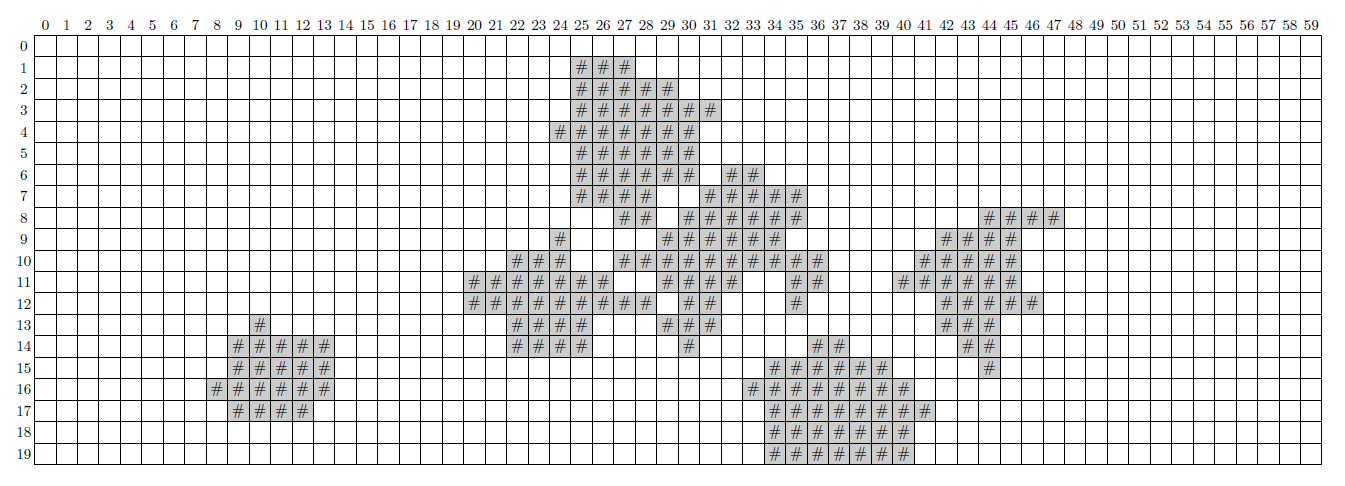
\includegraphics[scale=0.30]{koloniepikker/colony_bitmap.png}}
\caption{Bitmap gemaakt van een petriplaat. Deze bitmap is een rechthoekig rooster met 20 rijen en 60 kolommen, waarbij de bits die bedekt zijn door bacteri\"ele kolonies worden aangeduid door hekjes (\#). Deze bitmap telt zes gebieden van aangrenzende bezette bits, maar slechts vijf daarvan worden als kolonies beschouwd, omdat er \'e\'en gebied bits heeft die op de buitenste rand van de bitmap liggen.}
  \end{center}

\subsection*{Input}
\subsubsection*{Voorbeeldinput}
\begin{verbatim}
1
20 61 1
                                                            
                         ###                                
                         #####                              
                         #######                            
                        #######                             
                         ######                             
                         ###### ##                          
                         ####  #####                        
                           ## ######        ####            
                        #    ######       ####              
                      ###  ##########    #####              
                    #######  ####  ##   ######              
                    ######### ##   #      #####             
          #           ####   ###          ###               
         #####        ####    #     ##     ##               
         #####                    ######    #               
        ######                   ########                   
         ####                     ########                  
                                  #######                   
                                  #######     
\end{verbatim}
\subsection*{Output}
\subsubsection*{Voorbeeldoutput}
\begin{verbatim}
5 32.2
\end{verbatim}

\end{figure}